\documentclass[11pt]{article}

% Header -----------------------------------------------------------------------
\usepackage[utf8]{inputenc}
\usepackage{graphicx}
\usepackage{tikz}
\usepackage{geometry}
% \usepackage{siunitx}
\usepackage{hyperref}
\geometry{
a4paper,
left=10mm,
right=10mm,
top=10mm,
bottom=15mm
}

\usepackage{helvet}

\usepackage{booktabs}

\renewcommand{\rmdefault}{ptm}
\renewcommand{\familydefault}{\sfdefault}


% Set PATH
\newcommand{\PATH}{../..}

% Row i I
\newcommand{\rowiIheight}{.16\textheight}
\newcommand{\rowiIhjust}{1}
\newcommand{\rowiIvjust}{.5}

% Row i II
\newcommand{\rowiIIheight}{.1\textheight}
\newcommand{\rowiIIhjust}{.75}
\newcommand{\rowiIIvjust}{.5}

\pagestyle{empty}

% Begin document ---------------------------------------------------------------
\begin{document}

% Figure 1
\renewcommand{\figurename}{Figure}
\setcounter{figure}{0}

\begin{figure}

% Row 1
\begin{tikzpicture}
	\node[anchor=north west] at (0,0) {
		\includegraphics[height=\rowiIheight]{\PATH/analysis/BCB/full/umap_density.png}};
	\node[anchor=north east] at (\rowiIhjust,\rowiIvjust) {\textbf{\LARGE{A}}};
\end{tikzpicture}
\begin{tikzpicture}
	\node[anchor=north west] at (0,0) {
		\includegraphics[height=\rowiIheight]{\PATH/analysis/BCB/full/umap_patient.png}};
	\node[anchor=north east] at (\rowiIhjust,\rowiIvjust) {\textbf{\LARGE{B}}};
\end{tikzpicture}
\begin{tikzpicture}
	\node[anchor=north west] at (0,0) {
		\includegraphics[height=\rowiIheight]{\PATH/analysis/BCB/full/umap_outcome.png}};
	\node[anchor=north east] at (\rowiIhjust,\rowiIvjust) {\textbf{\LARGE{C}}};
\end{tikzpicture}


% Row 2
\begin{tikzpicture}
	\node[anchor=north west] at (0,0) {
		\includegraphics[height=\rowiIIheight]{\PATH/analysis/BCB/full/umap_libsize.png}};
	\node[anchor=north east] at (\rowiIIhjust,\rowiIIvjust) {\textbf{\LARGE{D}}};
\end{tikzpicture}
\begin{tikzpicture}
	\node[anchor=north west] at (0,0) {
		\includegraphics[height=\rowiIIheight]{\PATH/analysis/BCB/full/umap_percentMT.png}};
	\node[anchor=north east] at (\rowiIIhjust,\rowiIIvjust) {\textbf{\LARGE{E}}};
\end{tikzpicture}
\begin{tikzpicture}
	\node[anchor=north west] at (0,0) {
		\includegraphics[height=\rowiIIheight]{\PATH/analysis/BCB/full/counts_seurat2000_scVI_n30l1h128_umap_doublet-score.png}};
	\node[anchor=north east] at (\rowiIIhjust,\rowiIIvjust) {\textbf{\LARGE{F}}};
\end{tikzpicture}
\begin{tikzpicture}
	\node[anchor=north west] at (0,0) {
		\includegraphics[height=\rowiIIheight]{\PATH/analysis/BCB/full/counts_seurat2000_scVI_n30l1h128_umap_doublet-class.png}};
	\node[anchor=north east] at (\rowiIIhjust,\rowiIIvjust) {\textbf{\LARGE{G}}};
\end{tikzpicture}
\begin{tikzpicture}
	\node[anchor=north west] at (0,0) {
		\includegraphics[height=\rowiIIheight]{\PATH/analysis/BCB/full/umap_cellcycle.png}};
	\node[anchor=north east] at (\rowiIIhjust,\rowiIIvjust) {\textbf{\LARGE{H}}};
\end{tikzpicture}

% Row 3
\begin{tikzpicture}
	\node[anchor=north west] at (0,0) {
		\includegraphics[width=\textwidth]{\PATH/analysis/BCB/full/umap_level-3-scores.png}};
	\node[anchor=north east] at (.5,0) {\textbf{\LARGE{I}}};
\end{tikzpicture}

\caption{Cell type diversity in bronchoalveolar lavage (BAL) fluid in severe COVID-19. A--H) UMAP embedding of 320709 transcriptomes based on a 30 dimensional latent space of an scVI model trained on 2000 HVGs. Data points have been colored by density (A), patient (B), disease outcome (C), library size (number of mRNA counts per cell, D), percentage of counts from mitochondria (E), scDblFinder score (F) and classification (G), cell cycle classification (H). Numeric variables have been averaged across overlapping data points. I) Cell type scores (AUC) based on marker gene expression (see \href{https://nubes.helmholtz-berlin.de/s/id9rrKNeditKMmF}{table S1, level 3}) on cell embeddings (as A).}
\end{figure}

\clearpage

% Figure S1
\renewcommand{\figurename}{Supplementary Figure}
\setcounter{figure}{0}

\begin{figure}
\begin{tikzpicture}
	\node[anchor=north west] at (0,0) {
		\includegraphics[width=\textwidth]{\PATH/analysis/BCB/overview/sample-overview.png}};
	\node[anchor=north east] at (1,.5) {\textbf{\LARGE{A}}};
\end{tikzpicture}
\begin{tikzpicture}
	\node[anchor=north west] at (0,0) {
		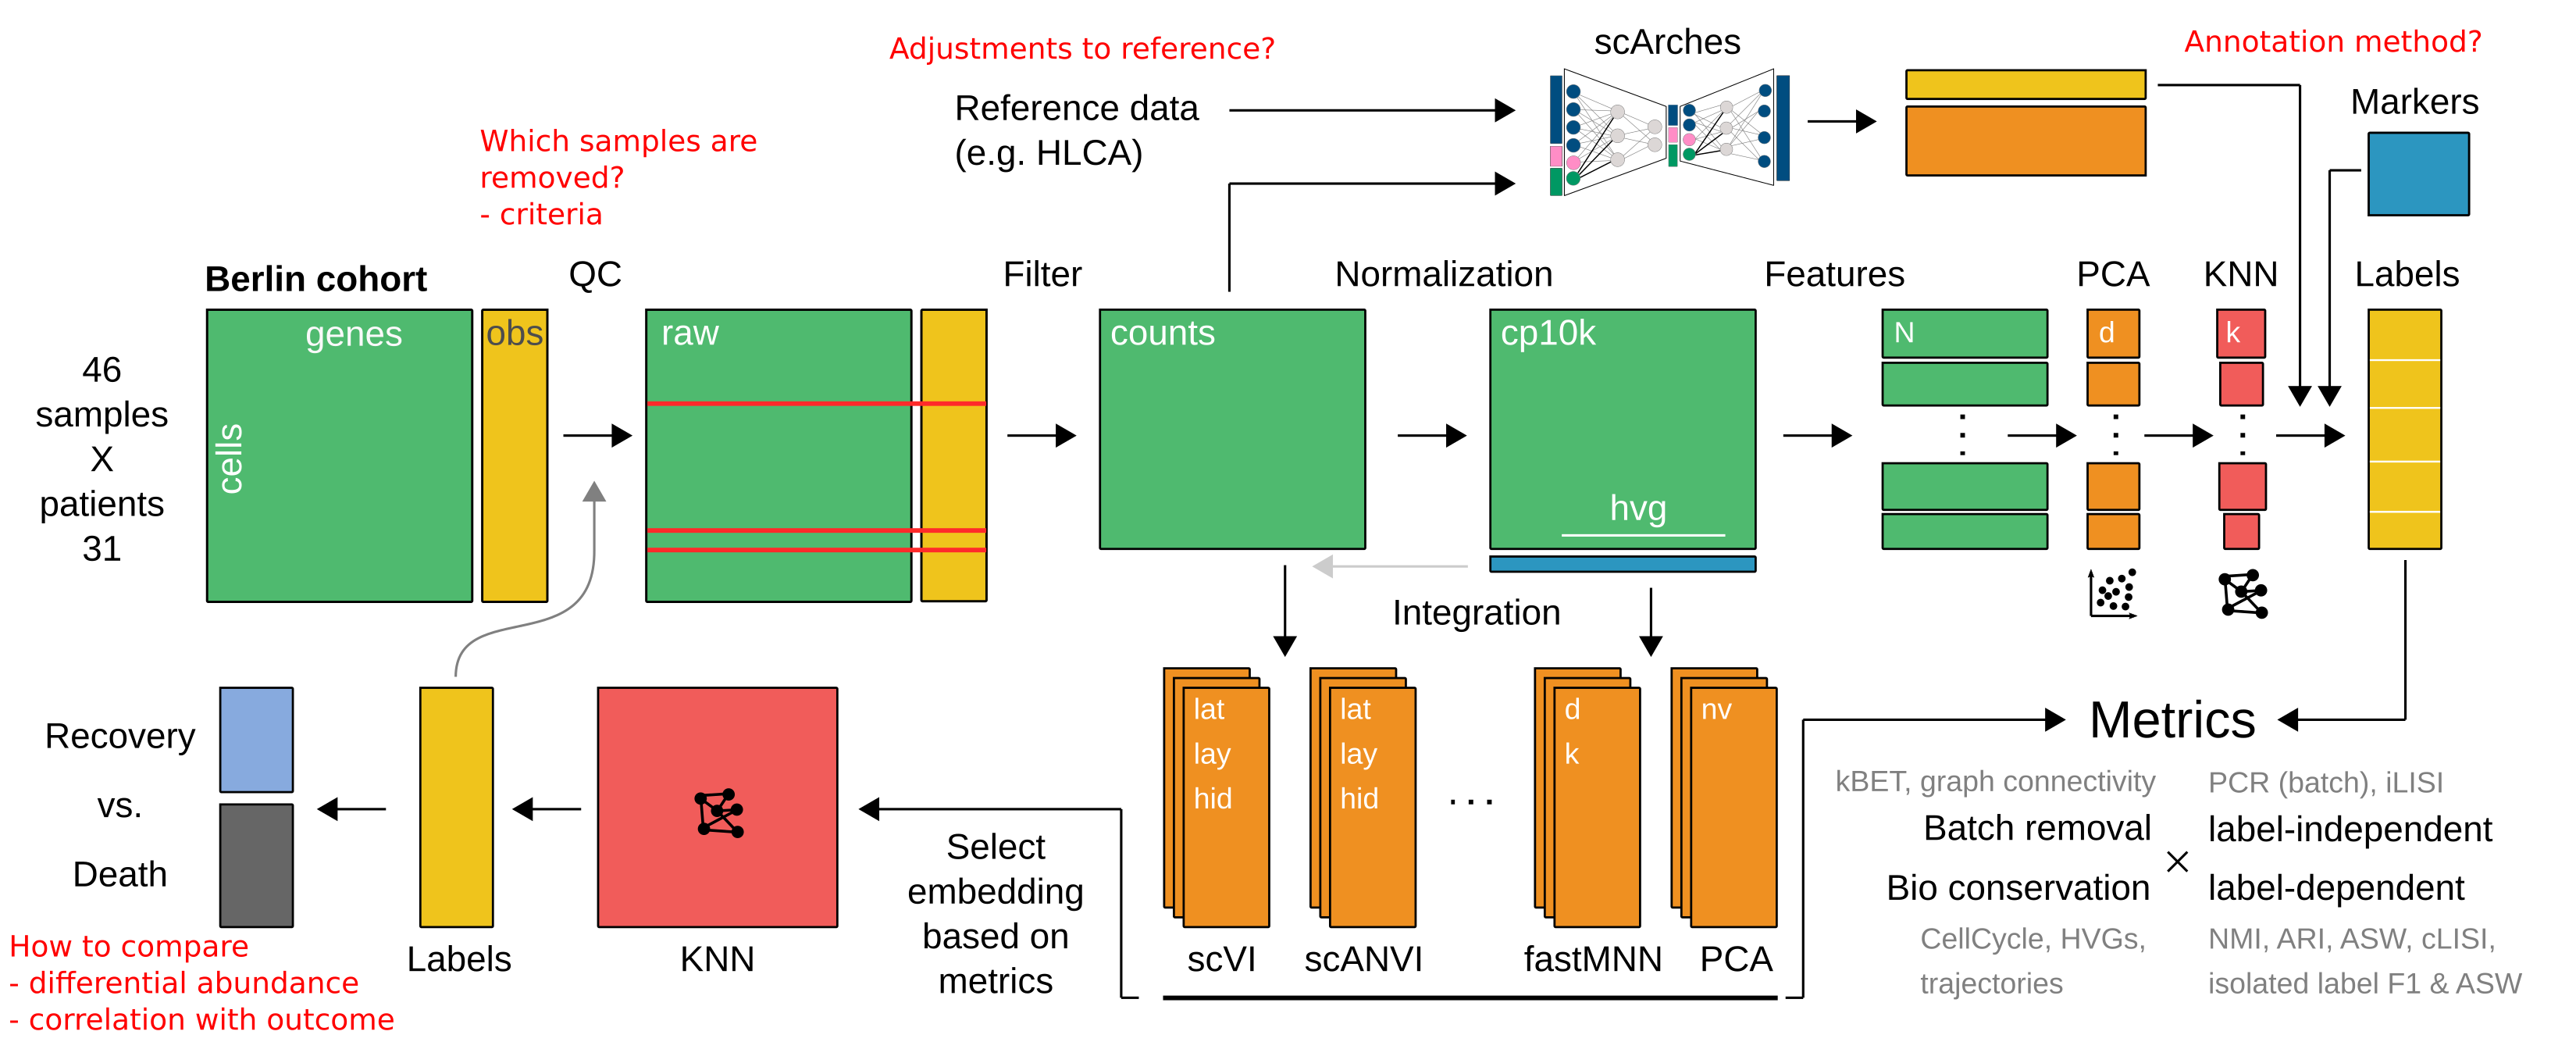
\includegraphics[width=\textwidth]{\PATH/docs/workflow/main.png}};
	\node[anchor=north east] at (1,-.5) {\textbf{\LARGE{B}}};
\end{tikzpicture}
\begin{tikzpicture}
	\node[anchor=north west] at (0,0) {
		\includegraphics[width=\textwidth]{\PATH/analysis/BCB/full/cluster-overview.png}};
	\node[anchor=north east] at (1,.5) {\textbf{\LARGE{C}}};
\end{tikzpicture}

\caption{Cell type diversity in bronchoalveolar lavage (BAL) fluid in severe COVID-19. A) Overview of the samples included in the dataset of BALs from severe COVID-19. B) Computational workflow for the analysis of BAL samples focused on the selection of the best integration method. Further, per-sample quality control and automated cell annotation are major goals. In the end, comparison of cellular composition across disease outcomes should lead to new insights.}
\end{figure}

\end{document}
